\documentclass[12pt,letterpaper]{article}
\usepackage[utf8]{inputenc}
\usepackage[spanish, russian]{babel}
\usepackage{amsmath}
\usepackage{amsfonts}
\usepackage{amssymb}
\usepackage{graphicx}
\usepackage[left=1cm,right=1cm,top=2cm,bottom=1cm]{geometry}
\author{Arthur Kupriyanov}

%Hipervinculos
\usepackage{hyperref}

\usepackage{listings}

%Color
\usepackage{color}
\definecolor{nred}{RGB}{174,49,54}
\definecolor{nblue}{RGB}{86,99,146}
\definecolor{nalgo}{RGB}{188,139,76}
\usepackage{sectsty}
\sectionfont{\color{nred}}
\subsectionfont{\color{nblue}}
\subsubsectionfont{\color{nalgo}}

%Cabeceras
\usepackage{fancyhdr}
\pagestyle{fancy}
\fancyhead[L]{Куприянов А.А}
\fancyhead[C]{Лабораторная работа №1}
\fancyhead[R]{НИУ ИТМО}


\newcommand{\R}{\mathbb{R}}
\newcommand{\Q}{\mathbb{Q}}
% \newcommand{\C}{\mathbb{C}}
\newcommand{\Z}{\mathbb{Z}}
\newcommand{\N}{\mathbb{N}}
% \newcommand{\U}{\mathbb{U}}
\newcommand{\Sol}{\mathbb{S}}
\newcommand{\M}{\mathbb{M}}
\newcommand{\X}{\mathbb{X}}

%Función, crea una matriz 3x4 con los corchetes ya puestos y la linea de separación entre A y b
%Se llama así \maa{1}{1}{1}{1}{2}{2}{2}{2}{3}{3}{3}{3}, esto va a crear una matriz donde la primera fila sean 1, la segunda solo 2 y la tercera 3, con los corchetes y la separación entre la matriz de las incognitas y el igual.
\newcommand{\maa}[8]{\left[ \begin{array}{ccc|c}
									#1 & #2 & #3 & #4\\
									#5 & #6 & #7 & #8\\
									\maacont}
\newcommand{\maacont}[4]{#1 & #2 & #3 & #4\\
							\end{array}\right]}	
							
%Otra función, crea una matriz columna 3x1 , la idea se esta función es enviar como primer parametro el igual, y el segundo y el tercero mostrar las modificaciones de las filas ex: \inter{=}{f_1 - f_2} {f_3 - f_1}					
\newcommand{\inter}[3]{\begin{array}{c}
#1\\
#2\\
#3\\
\end{array}}

\begin{document}

\begin{titlepage}
 
\begin{center}

{\Large {НИУ ИТМО} }
 

\includegraphics[scale=1]{bw_eng.jpg}
\\[1cm]

{\Huge \textsc{Лабораторная работа №1}}\\[0.7cm]
{\Huge Метод Гаусса}\\[2cm]

\begin{minipage}[l]{0.4\textwidth}
	\begin{flushleft}
		\textbf{\textsf{Преподаватель:}}\\
		\large Перл О.В.\\ 
% 		\linespread{4}

		\end{flushleft}
\end{minipage}
\begin{minipage}[l]{0.4\textwidth}

	\begin{flushright}
		\textbf{\textsf{Выполнил:}}\\
		\linespread{1}
		\large Куприянов А.А.\\
	\end{flushright}
\end{minipage}
 
\end{center}
 
\end{titlepage}


\section*{Описание метода}

Метод Гаусса состоит из двух основных этапов: прямой ход и обратный. \\
Прямой ход - это процесс нахождения коэффициентов треугольной системы, а обратный - это процесс получения неизвестных значений
переменных.
\begin{enumerate}
\section*{Прямой ход}



%%%%%%%%%%%%%%%%%%%%%%%%%%%%%%%%%%%%%%%%%%%%%%%%%%%%%%%%%%%%%%%%%%%%
%					Ejercicio	1							   %
%%%%%%%%%%%%%%%%%%%%%%%%%%%%%%%%%%%%%%%%%%%%%%%%%%%%%%%%%%%%%%%%%%%%
\item Допустим, у нас есть система трёх уравнений с тремя неизвестными

(1)  $\begin{array}{lcccccc}
		a_{11}x_{1} &+& a_{12}x_{2} &+& a_{13}x_{3} &=& a_{14}\\
		a_{21}x_{1} &+& a_{22}x_{2} &+& a_{23}x_{3} &=& a_{24}\\ 
		a_{31}x_{1} &+& a_{32}x_{2} &+& a_{33}x_{3} &=& a_{34}\\
\end{array}$

Пусть $a_{11} != 0$ (ведущий элемент). Исключим неизвестную $x_{1}$ из системы.

Разделив коэффициенты первого уравнения сиситемы (1) на $a_{11}$, мы получим:
\begin{center}
    (2) $\begin{array}{lcccccc}
        x_{1} &+& b_{12}x_2 &+& b_{13}x_4 &=& b_{15}
    \end{array}$ , где $b_{1j} = \frac{a_{1j}}{a_{11}}$
    \end{center}

Пользуясь этим уравнением (2) мы можем исключить из системы (1) неизвестную $x_1$. Нужно из второго уравнения системы (1) вычесть уравнение (2), умноженное на $a_{21}$, из третьего уравнения системы вычесть уравнение (2), умноженое на $a_{31}$

В результате получим систему уже двух уравнений:
\begin{center}
    $\begin{array}{lcccc}
		a_{22}^{(1)}x_{2} &+& a_{23}^{(1)}x_{3} &=& a_{24}^{(1)} \\ 
		a_{32}^{(1)}x_{2} &+& a_{33}^{(1)}x_{3} &=& a_{34}^{(1)} \\
\end{array}$
\end{center}

Выполнив такую операцию еще раз, мы придем к уравнению:

\begin{center}
    $x_3 = \frac{a_{34}^{(2)}}{a_{33}^{(2)}} = b_{34}^{3}$
\end{center}
\section*{Обратный ход}

\item Далее, мы можем последовательно определить остальные неизвестные из уравнений:

\begin{center}
\begin{flushleft}
    $x_2 = b_{24}^{(1)} - b_{23}^{(1)}x_3$ \\
    $x_1 = b_{14} - b_{13}x_3 - b_{12}x_2$
    \end{flushleft}
\end{center}

Таким образом, процесс решения линейной системы по методу Гаусса - это построение эквивалентной системы, имеющей треугольную матрицу.

\section*{Необходимое и достаточное условие}
Необходимым и достаточным условием применимости метода является, то что \\ ведущие элементы  не равны нулю

\end{enumerate}

\section*{Блок схема}
\begin{center}
    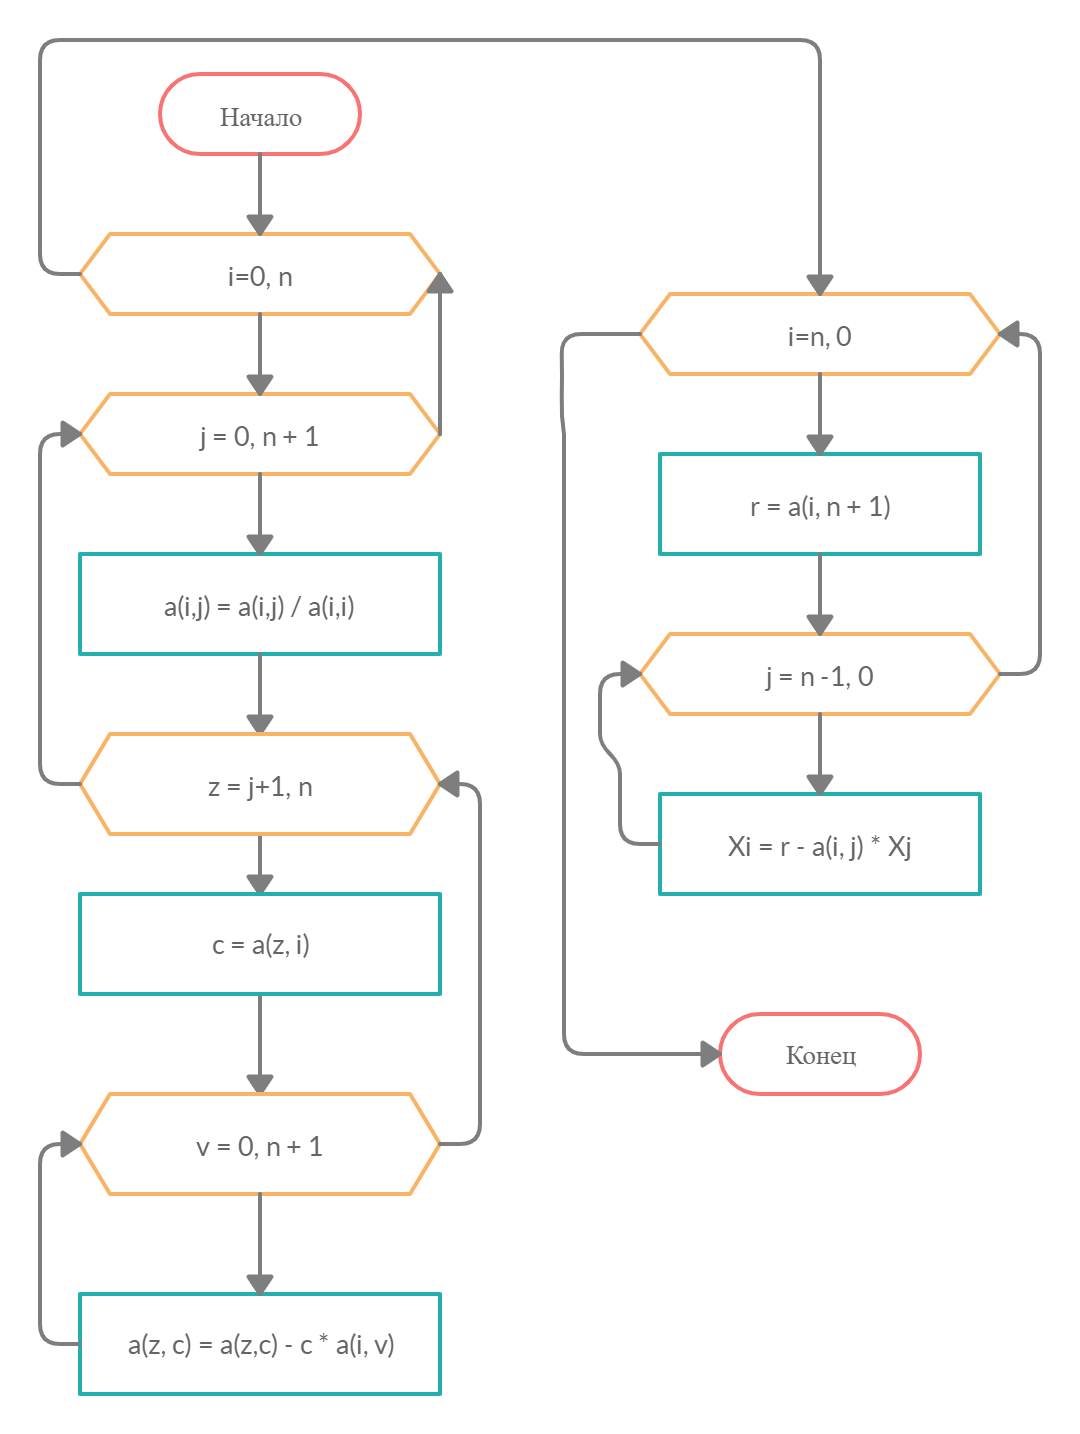
\includegraphics[scale=0.4]{1.jpg}
\end{center}

\newpage
\section*{Исходный код}
\begin{enumerate}
\item Прямой ход
\begin{lstlisting}[language=java]
public Matrix decompose(Matrix matrix) {
    for (int vIndex = 0; vIndex < matrix.getYSize(); vIndex++){
        float leadElement = matrix.getElement(vIndex, vIndex);
        float[] equation = makeEquation(matrix, leadElement, vIndex);
        bottomSubtract(matrix, vIndex, equation);
    }
    return matrix;
}

private float[] makeEquation(Matrix matrix, float leadElement, int vIndex){
    float[] equation = new float[matrix.getXSize()];
    for (int hIndex = 0; hIndex < matrix.getXSize(); hIndex++) {
        equation[hIndex] = matrix.getElement(vIndex, hIndex)/leadElement;
        matrix.setElement(vIndex, hIndex, equation[hIndex]);
    }
    return equation;
}

private void bottomSubtract(Matrix matrix, int vIndex, float[] equation){
  for (int z = vIndex + 1; z < matrix.getYSize(); z++) {
   float nextLeadElem = matrix.getElement(z, vIndex);
   for (int hIndex = 0; hIndex < matrix.getXSize(); hIndex++) {
     float value = matrix.getElement(z, hIndex)-nextLeadElem*equation[hIndex];
     matrix.setElement(z, hIndex,value);
   }
  }
}
\end{lstlisting}
Так как определитель матрицы при делении ее строки на ведующий элемент тоже делится на этот элемент и учитывая, то что
при вычитании из строк строки он не меняется - мы можем найти определитель матрицы во время прямого прохода:
\begin{center}
    $det(a_{ij}^{0}) = a_{11}^{(0)}a_{22}^{(1)} ... a_{nn}^{(n-1)}$
\end{center}
\newpage
\item Обратный ход
\begin{lstlisting}[language=java]
private float[] backSubstitution(Matrix matrix){
  float[] values = new float[matrix.getYSize()];
  for (int hIndex = matrix.getYSize() - 1; hIndex >= 0; hIndex--) {
      float rightValue = matrix.getElement(hIndex, matrix.getXSize() - 1);
      values[hIndex] = findVariable(matrix, hIndex, rightValue, values);
  }

  return values;
}

private float findVariable(
Matrix matrix,int hIndex,float initialValue,float[] previousVariables
) {
  float value = initialValue;
  for (int vIndex = matrix.getXSize() - 2; vIndex >= 0; vIndex--) {
    value =value-matrix.getElement(hIndex, vIndex)*previousVariables[vIndex];
  }
  return value;
}
\end{lstlisting}
\item Пример применения 

$\begin{array}{|lccccccccc}
13x_{1} &+& 15x_{2} &+& 13x_3 &+& 18x_4 &+& 13x_5 & = 16\\
12x_{1} &+& 12x_{2} &+& 16x_3 &+& 17x_4 &+& 13x_5 & = 15\\ 
14x_{1} &+& 18x_{2} &+& 16x_3 &+& 19x_4 &+& 17x_5 & = 14\\
18x_{1} &+& 16x_{2} &+& 18x_3 &+& 20x_4 &+& 18x_5 & = 16\\
19x_{1} &+& 15x_{2} &+& 18x_3 &+& 13x_4 &+& 15x_5 & = 18\\
\end{array}$

Решение: \\
x1: 0.789790, x2: 0.696697, x3: 0.818318, x4: 0.575075, x5: -1.977477, 

Невязка: \\
2.384186e-07, 3.725290e-08, 0.000000e+00, 0.000000e+00, 0.000000e+00
\end{enumerate}

\section*{Вывод}

Как видно из реализации, в этом методе, если в прямом ходе окажется ведущий элемент равный нулю, то этот вариант метода Гаусса не пригоден. Альтернативным вариантом является метод Гаусса с выбором главного элемента. Это более универсальный метод, но медленее. По сути, метод Гаусса, является частным случаем метода главных элементов

Рассмотренный метод также имеет недостаток в тех случаях, когда ведущие элементы будут иметь маленькую величину. Из-за специального представления чисел в ЭВМ существует машинная погрешность, что катастрафически может увеличить погрешность при очень малых значениях элементов. Так, например, в этой лабораторной работе была использована JDK 1.8 HotSpot, которая в своей виртуальной машине поддерживала float value set: 24 бит под мантиссу и еще 8 под знак и смещенную экспоненту, итого 4 байта
\end{document}